\clearpage
\section{Forschungsteil}
\label{sec:work}

Um die Frage zu beantworten, ob es bestimmte Hänge zu einem oder dem anderen Paradigma gibt, muss zuerst beantwortet werden, wie die Paradigmen mit den Lerntypen zusammenhängen. 
Hierzu wird betrachtet, welche Lerntypen Vorteile beim Lernen der Computational Thinking (CT) Aspekte haben könnten. Außerdem wird geprüft, welche Empfehlungen für die Lerntypen laut Felder und Silvermann mit den Eigenschaften der Paradigmen zusammenhängen können. Hierbei wird Objektorientierung (OO) als häufigstes Paradigma in Einführungskursen, sowie funktionale Programmierung (FP) als Fokuspunkt der Arbeit betrachtet. Andere Programmierparadigmen werden zunächst ausgelassen. Abschließend wird evaluiert, welche Rolle die CT Aspekte in den unterschiedlichen Paradigmen haben, um zu bestimmen, ob ein Vor- oder Nachteil für ein Paradigma möglicherweise besonders ausgeprägt ist.

% Disclaimer
Es werden hierbei vermehrt Annahmen zu den Vorlieben der Lerntypen gemacht, aufgrund der Empfehlungen von Felder und Silvermann in Relation zu den Merkmalen der Paradigma. Aufgrund der zeitlichen Beschränkung der Arbeit können diese Annahmen nicht empirisch überprüft werden.

\subsection{Lerntypen im Zusammenhang mit Computational Thinking}
Programmierkenntnisse zu erlernen bedeutet nicht nur Code zu schreiben, sondern auch CT Kompetenzen zu erwerben.
Nicht jede Lerntypen Dimension zeigt Vor- oder Nachteile beim Lernen der CT Aspekte, allerdings lassen sich einige klare Zusammenhänge herausstellen.

\subsubsection{Auditiv Visuell}
Visuelle Lerner können einen Vorteil beim Erlernen von Abstraktion haben, da grafische Darstellungen eine sehr geeignete und beliebte Form sind, um das Konzept von Abstraktion zu erklären. Beispielsweise in der Objektorientierung werden hierbei öfters Bilder von Objekten wie Tieren oder Fahrzeugen verwendet, die dann auf Codeblöcke abstrahiert werden.
Allerdings lässt sich auch notieren, dass verbale Lerntypen generell einen Vorteil in herkömmlichen Vorlesungen haben, da diese meist mit einem frontalen Input gehalten werden. Welche Lerntypen hier einen Vorteil haben, hängt von daher eher davon ab, zu welchen Darstellungsformen sich der Dozent letztenlich entscheidet. % QUELLE? Also spezifische Frage, könnte man hier einfach einen Vorlesungsblock finden oder einen Artikel?

\subsubsection{Reflektiv Aktiv}
Reflektive Lerner könnten einen klaren Vorteil im Aspekt Debugging haben. Sie sind eher dazu veranlagt, ihre gefundenen Lösungen zu evaluieren, und zu hinterfragen. Es ist demnach wahrscheinlicher, dass ein reflektiver Lerner von Natur aus Konzepte des Debugging anwendet. Aktive Lerner hingegen sind risikobereiter, und sind in ihrer Arbeit experimentierfreudiger. Hierbei gilt eher der Ansatz, schneller zu scheitern, aber auch dafür schneller wieder neue Lösungen auszuprobieren.

\subsubsection{Sensorisch Intuitiv}
Intuitive Lerner haben einen expliziten Vorteil im Aspekt der Abstraktion \cite{felderhandout}. Dies ist der Fall unter anderem, da sie sich eher mit Konzepten statt Auswendiglernen beschäftigen. Intuitive Typen meiden normalerweise Kurse, die zum Großteil aus Auswendiglernen und Formeln anwenden bestehen, und ziehen neue Theorien und Interpretationen vor. % TODO Formulierung
Auch im Algorithmischen Denken werden Personen mit einem Hang zu intuitivem Lernen einen Vorteil haben, da sie normalerweise Konzepte schneller lernen als sensorische Lerner. Sie ziehen Innovation den etablierten Methoden vor, und meiden eher Repitition. Dies könnte im Aspekt des Algorithmischen Denken von Vorteil sein, um neue Ansätze für Probleme zu entwickeln. Besonders im Zusammenhang mit dem Aspekt des Debuggens, könnte dies zu schnelleren und effizienteren Lösungen führen.

\subsubsection{Sequentiell Global}
In dieser Lerndimension lässt sich ein Vorteil für sequentielle Lerntypen im Aspekt der Dekomposition erkennen. Das Herunterbrechen auf Teilprobleme ist nicht nur ein wichtiger CT Aspekt, sondern auch eine Veranlagung des sequentiellen Lerntypen, der es vorzieht, Probleme in einem "Step by Step" Ansatz anzugehen. Sie beschäftigen sich mit allen Teilproblemen, bevor sie die komplette Lösung etwickeln können. Sequentielle Lerner brauchen kein Bild vom großen und ganzen, um die einzelnen Teile angehen zu können, und haben daher einen entscheidenen Vorteil im Herunterbrechen der Teilprobleme im Vergleich zu globalen Lerntypen.

\subsection{Eignung der Lerntypen für die Programmierparadigmen}
Auch bei den Lerntypen des Felder Silvermann Modelles lassen sich teilweise Hänge zu einem bestimmten Paradigma erkennen.

\subsubsection{Auditiv Visuell}
Hinsichtlich der Unterscheidung zwischen visuellen und auditiven Typen lässt sich beidseitig argumentieren. Beim Erlernen von Objektorientierten Konzepten wie Vererbung bieten sich visuelle Darstellungen wie Graphen an, ähnlich wie im Aspekt der CT Abstraktion.
Allerdings können visuelle Typen auch einfacher mathematische Konzepte und Formeln auf die Philosophien der funktionalen Programmierung übertragen, und die Zusammenhänge besser verstehen. Da FP einen starken Zusammenhang mit der Mathematik hat, können durch gewohnte Strukturen von Formeln und Funktionen einfachere Parallelen gezogen werden.
Welcher Lerntyp hier einen besseren Vorteil hat, kommt allerdings sehr auf die Strukturierung der Vorlesung an.

\subsubsection{Reflektiv Aktiv}
In der aktiven und reflektiven Dimension lässt sich in beiden betrachteten Paradigmen ein Vorteil für den reflektiven Typen erkennen. Die praktische Umsetzung von Programmierkenntnissen erfolgen meistens in Einzelarbeit, und erfordern eine stetige Reflektion des Lerners.
Das Erlernen von Programmierkenntnissen könnte theoretisch auch in Gruppenarbeiten erfolgen, allerdings werden die meisten Vorlesungsstile reflektiven Typen einen Vorteil bieten.

\subsubsection{Sensorisch Intuitiv}
Hierbei zeigt sich ein deutlicher Hang zu den Paradigmen. Sensorische Typen werden höchstwahrscheinlich OO bevorzugen. Die Klassen der OO modellieren Objekte der echten Welt, und haben somit einen einfach verständlichen Bezug zu echten Problemen.
Intuitive Typen hingegen sind besser darin, Abstraktion anzuwenden, und werden daher eher FP bevorzugen. Sie können aufgrund ihres Hanges zu Innovation und Verständnis von abstrakteren Konzepten ohne direkten Bezug zur echten Welt schneller Konzepte der FP verstehen und umsetzen. Die deklarative Art, wie FP aufgebaut ist bietet diesem Lerntypen einen eindeutigen Vorteil.

\subsubsection{Sequentiell Global}
Auch in der sequentiell globalen Dimension lassen sich klare Zusammenhänge zu den Paradigmen erkennen. Globale Lerntypen werden es höchstwahrscheinlich vorziehen, zunächst über eine OO Klasse als Ganzes nachzudenken, bevor sie sich mit der Implementierung von Details beschäftigen. Um eine sinnvolle Hierarchie zur Komposition der verschiedenen Klassen zu entwerfen, muss grundlegend ein globaleres Verständnis der Problemes vorhanden sein.
Sequentielle Typen hingegen werden eher FP bevorzugen, da das Paradigma das Herunterbrechen von Problemen in Teilschritte von Grund auf vorsieht. Die Probleme werden in Teilfunktionen behandelt, und erst zum Schluss ergibt sich der Zusammenhang zu einem Programm. Es muss nicht direkt ein globales Verständnis der Lösung vorhanden sein, sondern die Lösung setzt sich eher aus den Teilproblemen zusammen.

\subsection{Ausprägung der Computational Thinking Aspekte in den Programmierparadigmen und Bezug zu Funktionaler Programmierung}
Um die Zusammenhänge zwischen den Vor- und Nachteilen herzustellen, muss betrachtet werden, wie genau die einzelnen CT Aspekte in dem Paradigmen ausgeprägt sind. Kein Aspekt kann in einem Paradigma vollständig ausgelassen werden, da CT generell für das Konzept des Programmierens benötigt wird. Allerdings beeinflussen die unterschiedlichen Schwerpunkte und Philosophien der Paradigma, wie die Aspekte gewertet und gewichtet werden können. 
Aufgrund dieser Analyse können dann zusätzliche Schlüsse und Wichtungen der Vor- und Nachteile der Lerntypen gezogen werden.
% Hierzu wurde keine Forschung gefunden, deswegen sind das alles eigene Schlüsse (Fazitmaterial)

\subsubsection{Dekomposition}
In der FP ist die Dekomposition sehr stark ausgeprägt. Jede Funktion hat nur eine einzige Verantwortung, und gibt immer das selbe Ergebnis wieder. Durch Vermeidung von Seiteneffekten ist die Funktionsweise jeder Methode eindeutig. Der Programmablauf ist eher eine Abfolge von Befehlen, als in der OO. In der OO erfolgt die Dekomposition nicht zwingenderweise auf Funktionsebene, sondern eher durch die einzelnen Klassen, und deren Verantwortung.
\\
Da in der FP die Dekomposition einen starken Fokus hat, könnten hierbei visuell Lerntypen einen zusätzlichen Vorteil hinsichtlich des funktionalen Paradigma mit sich bringen.

\subsubsection{Abstraktion}
Die Abstraktion in OO ist generell einfach zu visualisieren. Meistens werden die Probleme auf Klassen mit jeweils eigenen Funktionen heruntergebrochen. Diese Klassen wiederum können in Diagrammen oder Bildern mit ihren Funktionen dargestellt werden.
In der Dekomposition der FP hingegen gibt es eine starke Kopplung mit der Dekomposition. Es gibt eine sehr starke Abstraktion bis hin zu mathematischen Funktionen.
\\
Da intuitive Typen tendenziell einen Vorteil in Abstraktion haben, könnten diese einen Vorteil in der Erlernung von FP allgemein haben.

\subsubsection{Algorithmen}
Bei der Entwicklung von Algorithmen gibt es in der OO je nach Sprache ein großes Toolset. Beispielsweise in Java sind Integer eine eigene Klassen, mit jeweils eigenen Operationen, die bei der Entwicklung verwendet werden können. In der FP hingegen ist das Toolset deutlich begrenzter, auch ein Abwesen an Zuständen im Code.
\\
Da in der FP Innovation bei der Entwicklung neuer Algorithmen sehr stark ausgeprägt ist, könnte ein Intuitiver Lerntypus hier einen besonderen zusätzlichen Vorteil haben.

\subsubsection{Debugging}
In der OO gibt es häufiger ein "klassisches" Debuggen. Klassen können diesen Prozess möglicherweise unübersichtlicher machen, als in der FP. FP hat eine besondere Sicht auf das Debuggen, da ein besonders hoher Wert auf die Fehlermeidung gelegt wird. Durch die eindeutige Verantwortung jeder Funktion, treten weniger Flüchtigkeitsfehler oder unbeabsichtigte Seiteneffekte auf. Tendenziell braucht Code, der mit funktionalen Sprachen geschrieben ist weniger nachträgliche Bugfixes.

\begin{figure}[h!]
    \centering
    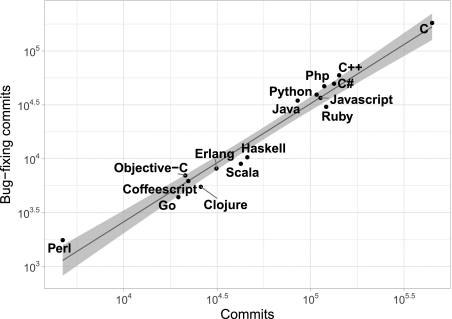
\includegraphics[width=1\linewidth]{Figures/FigBugCommitsFP}
    \caption{Commits und Bugfixing-Commits in verschiedenen Programmiersprachen \cite{berger}}
\end{figure}

Aufgrunde der besonders ausgeprägten Anforderung an die Reflektion beim Schreiben des Codes, haben sequentielle Typen möglicherweise einen zusätzlichen Vorteil in der FP. Funktionen werden sequentiell evaluiert und geschrieben, und benötigen nicht so stark ein globales Verständnis des Problemes wie vergleichsweise in der OO.

\subsection{Zusammenfassung}
Zusammengefasst lassen sich also definitiv gewisse Vorteile mancher Lerntypen erkennen. In diesem Abschnitt werden die Vorteile besonders im Hinblick auf die FP betrachtet.

\begin{figure}[h!]
    \centering
    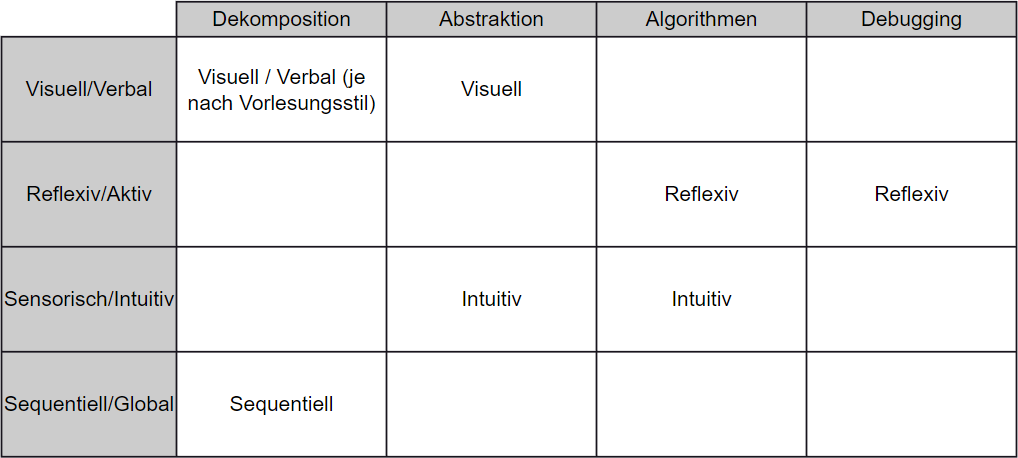
\includegraphics[width=1\linewidth]{Figures/Section_3/Styles_CT}
    \caption{Vorteile der Lerntypen in den Aspekten des Computational Thinking}
\end{figure}

Für die Computational Thinking Aspekte lässt sich zusammenfassend sagen, dass besonders Personen mit Visuell, Reflektiv, Intuitiv und Sequentiell ausgeprägten Veranlagungen einen Vorteil beim Erlernen der CT Aspekte haben werden.

\begin{figure}[h!]
    \centering
    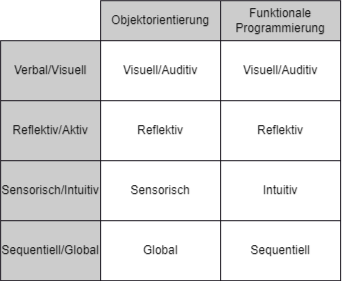
\includegraphics[width=1\linewidth]{Figures/Section_3/Styles_Paradigms}
    \caption{Vorteile der Lerntypen in den betrachteten Paradigmen}
\end{figure}

Für die Computational Thinking Aspekte lässt sich zusammenfassend sagen, dass besonders Personen mit Reflektiv, Intuitiv und Sequentiell ausgeprägten Veranlagungen Vorteile beim Lernen mit funktionaler Programmierung haben werden.
Personen mit Reflektiv, Sensorischen und Global ausgeprägten Eigenschaften hingegen werden besser mit OO Programmierung lernen.

\begin{figure}[h!]
    \centering
    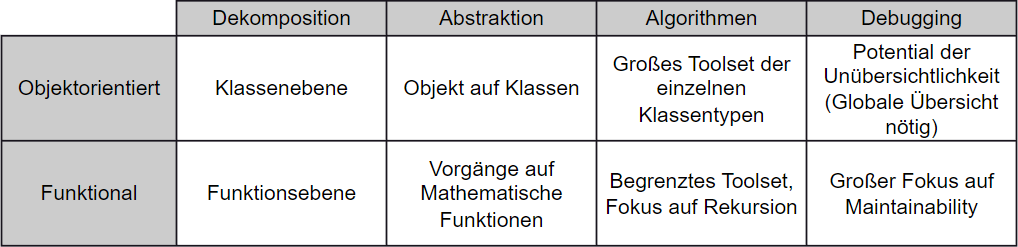
\includegraphics[width=1\linewidth]{Figures/Section_3/CT_Paradigms}
    \caption{Ausprägungen der CT Aspekte in den jeweiligen Programmierparadigmen}
\end{figure}

Zu den einzelnen Ausprägungen der CT Aspekte in den Paradigmen lassen sich zusätzliche Vorteile der Lerntypen ziehen. So hat beispielsweise ein sequentieller Lerntypus einen besonderen Vorteil in der FP, da sowohl das Debugging eine hohe Wichtigkeit in der FP hat, und der Typus generell einen Vorteil bei der Erlernung von Debugging als CT Aspekt hat.

\subsubsection{Vor- und Nachteile der Lerntypen hinsichtlich Funktionaler Programmierung}
Durch die Analyse sowohl der Programmierparadigmen, als auch der Computational Thinking Aspekte hinsichtlich der Lerntypen haben sich klare Vorteile einiger Ausprägungen ergeben.
Insbesondere folgende Lerntypen werden demnach \textbf{Vorteile} haben, wenn sie ihren Programmiereinstieg mit funktionaler Programmierung machen.

\begin{description}
    \item[Visuell] Da ein direkter Bezug zu mathematischen Formeln gemacht werden kann. Zudem haben visuelle Typen einen Vorteil in der Dekomposition.
    \item[Reflektiv] Da Programmierung tendenziell eher in Einzelarbeit erfolgt, und der Lerntypus in herkömmlichen Vorlesungsstilen besser unterstützt werden kann. Zudem hat der reflektive Lerntypus einen Vorteil im Erlernen des Debugging als CT Aspekt.
    \item[Intuitiv] Da dieser Typus in der FP einen besonderen Vorteil in der Abstraktion hat, die in der FP eine hohe Wichtigkeit hat, da die meisten funktionalen Programmiersprachen eine theoretische Basis im Lambda Kalkül haben. Auch bei der Innovation hinsichtlich neuer Algorithmen, was in der FP besonders relevant ist, hat dieser Typ einen Vorteil.
    \item[Sequentiell] Da FP einen eher sequentiell veranlagten Entwicklungsstil hat, in dem ein Teilproblem nach dem Anderen angegangen wird. Zudem kann eine sequentielle Veranlagung zusätzlich bei der Erlernung von Dekomposition helfen.
\end{description}

Diese Ausprägungen decken sich zudem mit dem ausgearbeiteten Vorteilen zum Erlernen von CT Aspekten, was einen zusätzlichen Vorteil bieten kann.
\\
Andererseits haben im Umkehrschluss wiederum folgende Lerntypen eher \textbf{Nachteile} bei FP.

\begin{description}
    \item[Verbal] Da verbal schwieriger ein Bezug zu den mathematischen Grundlagen von FP gemacht werden kann.
    \item[Aktiv] Da Programmierung allgemein reflektive Typen zu bevorzugen scheint. Zudem wiederspricht ein aktiver Stil der Wichtigkeit des Debuggings in der FP.
    \item[Sensorisch] Da nicht so ein guter Bezug zu echten Problemen hergestellt werden kann. Zudem hat ein sensorischer Typ eher Nachteile beim Erlernen von Abstraktion, und beim innovativem Ausarbeiten von neuen Lösungen für Probleme. Das anwenden etablierter Methoden ist besonders beim Erlernen von FP schwieriger, da sich das Paradigma von anderen Programmierstilen stark unterscheidet.
    \item[Global] Da eher ein sequentielles Denken gefordert ist. In der OO ist ein globales Denken von Vorteil, da der Zusammenhang zwischen den Domänen eine Rolle spielt, in der FP allerdings werden die Probleme eher "Step by Step" angegangen, was für diesen Lerntypen ein Nachteil sein könnte.
\end{description}